\section{Physical/Deployment View}

Die \textit{Physical View} beschreibt die Anordnung der Komponenten.
Sie stellt die Topologie und Kommunikation zwischen den Komponenten dar. 
Da das Projekt über Kubernetes bereitgestellt wird, zeigt diese physische Ansicht das Projekt in einem Kubernetes-Cluster an.
Die Physical View ist in \autoref{fig:component} zu sehen.

\begin{figure}[h]
    \centering
   \makebox[0pt]{%
    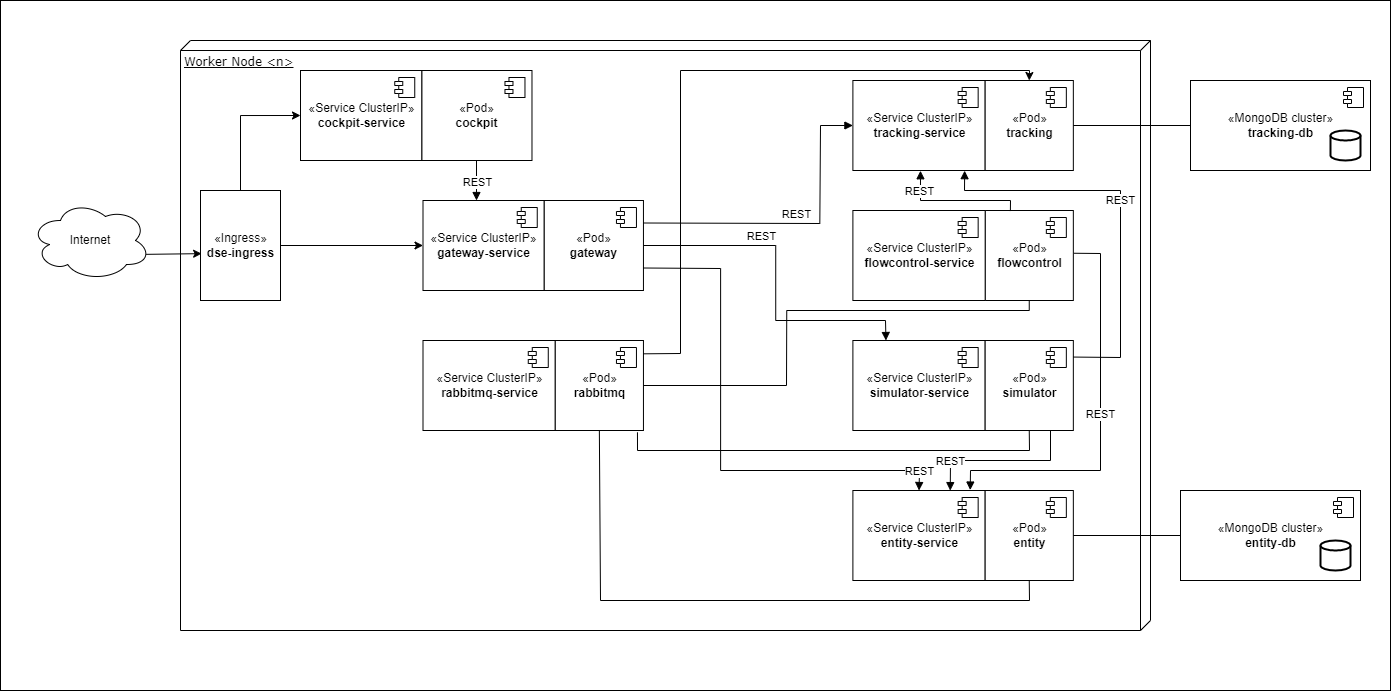
\includegraphics[width=20cm]{./figures/component_diagram.png}}
    \caption{Komponentendiagramm}
    \label{fig:component}
\end{figure}
